\begin{figure}[htbp]
  \centering
  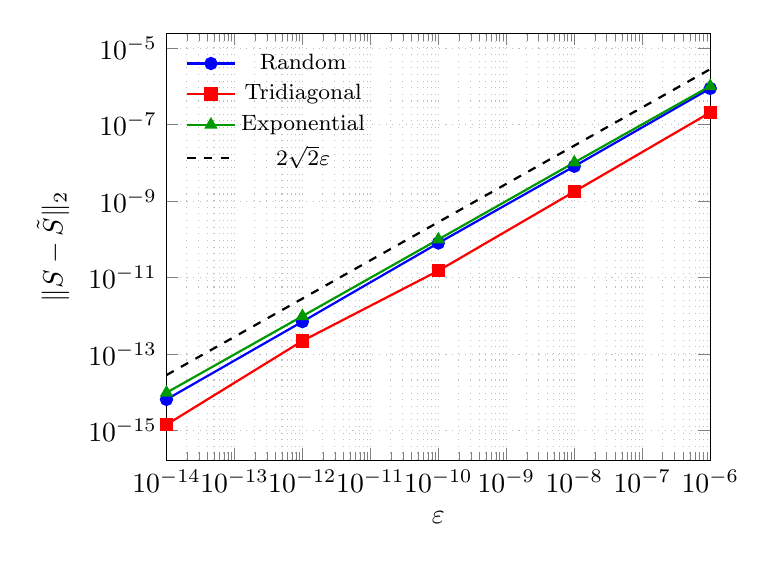
\begin{tikzpicture}
  \begin{axis}[
      width=0.7\linewidth,
      height=7.0cm,
      xmode=log,
      ymode=log,
      log basis x=10,
      xlabel={$\varepsilon$},
      ylabel={$\|S-\tilde S\|_2$},
      grid=both,
      grid style={dotted},
      minor tick num=0,
      enlarge x limits=false,
      legend style={
          font=\footnotesize,
          draw=none,
          fill=none,
          at={(0.02,0.98)},
          anchor=north west
      }
  ]

  % --- Random ---
  \addplot[blue, thick, mark=*] coordinates {
  (1.000000e-14, 6.521864e-15) (1.000000e-12, 7.052797e-13) (1.000000e-10, 8.019122e-11) (1.000000e-08, 8.152643e-09) (1.000000e-06, 8.868481e-07) 
  };
  \addlegendentry{Random}

  % --- Tridiagonal ---
  \addplot[red, thick, mark=square*] coordinates {
  (1.000000e-14, 1.427078e-15) (1.000000e-12, 2.214184e-13) (1.000000e-10, 1.513407e-11) (1.000000e-08, 1.776349e-09) (1.000000e-06, 2.080670e-07) 
  };
  \addlegendentry{Tridiagonal}

  % --- Exponential ---
  \addplot[green!60!black, thick, mark=triangle*] coordinates {
  (1.000000e-14, 9.788353e-15) (1.000000e-12, 9.813416e-13) (1.000000e-10, 9.946941e-11) (1.000000e-08, 1.022867e-08) (1.000000e-06, 1.015741e-06) 
  };
  \addlegendentry{Exponential}

  % --- Theoretical bound ---
  \addplot[black, dashed, thick, mark=none] coordinates {
  (1.000000e-14, 2.828427e-14) (1.000000e-06, 2.828427e-06) 
  };
  \addlegendentry{$2\sqrt{2}\varepsilon$}

  \end{axis}
  \end{tikzpicture}
  \caption{Perturbation error versus $\varepsilon$ ($N=8$).}
  \label{fig:err_vs_eps}
\end{figure}


\begin{figure}[htbp]
  \centering
  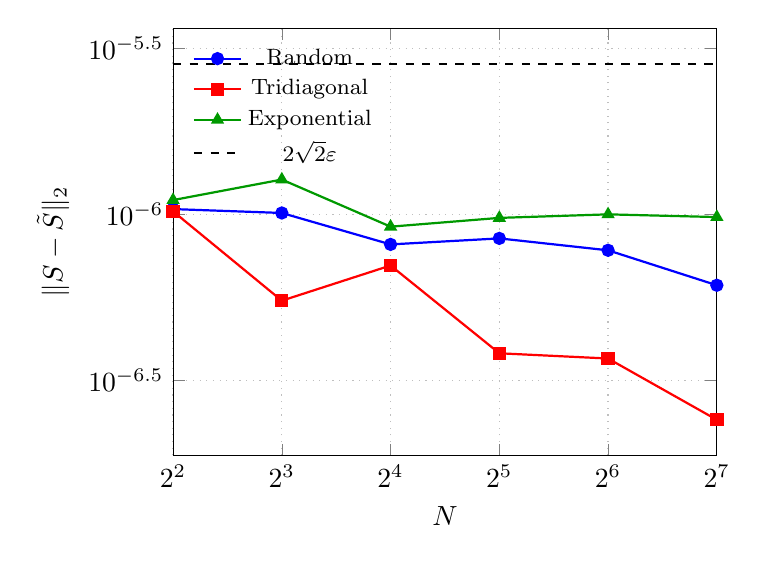
\begin{tikzpicture}
  \begin{axis}[
      width=0.7\linewidth,
      height=7.0cm,
      xmode=log,
      ymode=log,
      log basis x=2,
      xlabel={$N$},
      ylabel={$\|S-\tilde S\|_2$},
      grid=both,
      grid style={dotted},
      minor tick num=0,
      enlarge x limits=false,
      legend style={
          font=\footnotesize,
          draw=none,
          fill=none,
          at={(0.02,0.98)},
          anchor=north west
      }
  ]

  % --- Random ---
  \addplot[blue, thick, mark=*] coordinates {
  (4.000000e+00, 1.036912e-06) (8.000000e+00, 1.009293e-06) (1.600000e+01, 8.116716e-07) (3.200000e+01, 8.462596e-07) (6.400000e+01, 7.793250e-07) (1.280000e+02, 6.115727e-07) 
  };
  \addlegendentry{Random}

  % --- Tridiagonal ---
  \addplot[red, thick, mark=square*] coordinates {
  (4.000000e+00, 1.020794e-06) (8.000000e+00, 5.495799e-07) (1.600000e+01, 7.013596e-07) (3.200000e+01, 3.817600e-07) (6.400000e+01, 3.680882e-07) (1.280000e+02, 2.406628e-07) 
  };
  \addlegendentry{Tridiagonal}

  % --- Exponential ---
  \addplot[green!60!black, thick, mark=triangle*] coordinates {
  (4.000000e+00, 1.103605e-06) (8.000000e+00, 1.272339e-06) (1.600000e+01, 9.178659e-07) (3.200000e+01, 9.755029e-07) (6.400000e+01, 9.996382e-07) (1.280000e+02, 9.810714e-07) 
  };
  \addlegendentry{Exponential}

  % --- Theoretical bound ---
  \addplot[black, dashed, thick, mark=none] coordinates {
  (4.000000e+00, 2.828427e-06) (1.280000e+02, 2.828427e-06) 
  };
  \addlegendentry{$2\sqrt{2}\varepsilon$}

  \end{axis}
  \end{tikzpicture}
  \caption{Perturbation error versus $N$ ($\varepsilon=1.0e-06$).}
  \label{fig:err_vs_N}
\end{figure}
